\documentclass[11pt]{article}
\usepackage{amsmath,amsfonts}
\usepackage[numbers,sort&compress]{natbib}
\usepackage{times}
\usepackage[left=2.54cm,top=2.54cm,right=2.54cm,bottom=2.54cm,bindingoffset=0.0cm]{geometry}
\usepackage{setspace}
\usepackage{enumerate}
\usepackage{enumitem}
\usepackage{wrapfig}
\setcounter{secnumdepth}{0}
\usepackage{fullpage}
\usepackage{titlesec}
\titleformat{\section}{\large\bfseries}{\thesection}{1em}{}
\titleformat{\subsection}{\bfseries}{\thesubsection}{1em}{}
\usepackage{parskip} % skip paragraph indentations
\usepackage{lipsum}
\usepackage{hyperref}
\usepackage{graphicx}
\usepackage{amssymb}
\usepackage[x11names]{xcolor}
\usepackage{hyperref}
\usepackage{enumitem}
\usepackage{booktabs}
\usepackage{amsmath}
\usepackage{amssymb}
\usepackage{mathrsfs}
\usepackage{caption} \captionsetup[table]{singlelinecheck=false} %makes table captions left-justified
\usepackage{framed} % to add frames around comments
%\hypersetup{backref,colorlinks=false,
%    urlbordercolor=LightSkyBlue4,          % color of internal links
%    citebordercolor=SpringGreen4,        % color of links to bibliography
%    filebordercolor=magenta,      % color of file links
%    linkbordercolor=Red3, pdfborderstyle={/S/U/W 1.5}}
\newcommand{\Prob}[1]{\Pr{\left( #1 \right)}}
\newcommand{\q}[1]{``#1''} % easier way to get double quotes
\newcommand{\argmin}{\text{argmin}}
\usepackage{authblk} % for title page
\renewcommand\Affilfont{\fontsize{10}{10.8}\itshape}
\renewcommand\familydefault{\sfdefault} 
\usepackage{datetime2}
%\renewcommand{\dateseparator}{-}
\usepackage{atbegshi}% http://ctan.org/pkg/atbegshi -- removes blank page at start of doc
\AtBeginDocument{\AtBeginShipoutNext{\AtBeginShipoutDiscard}}
\setcounter{page}{0}
\begin{document}
\noindent
\title{Draft: Learned badges vs. Social recognition} 
%The evolution of rank signaling?

\author[1]{Eleanor Brush}
\affil[1]{University of Maryland; email: xxxxx}
\author[2,3,4]{Elizabeth A. Hobson}
\affil[2]{Santa Fe Institute, 1399 Hyde Park Road, Santa Fe, NM 87501 USA}
\affil[3]{Center for Biosocial Complex Systems, Arizona State University}
\affil[4]{National Institute for Mathematical and Biological Synthesis, University of Tennessee, Knoxville, TN, USA; email: ehobson@santafe.edu}
%\date{} 
\maketitle

Target journal: Behavioral Ecology 
%instructions: http://www.oxfordjournals.org/our_journals/beheco/for_authors/general.html
% also: http://www.oxfordjournals.org/our_journals/beheco/for_authors/submission_online.html

Target submission date: October? or maybe early November??
%%%%%%%%%%%%%%%%%%%%%%%
\linenumbers
%%%%%%%%%%%%%%%%%%%%%%%

\section*{Abstract}

\framebox(500,100){to be added..........................................}

\textit{Keywords: signal evolution, cognition, social groups, [.....]}
\newline

%%%%%%%%%%%%%%%%%%%%%%%
\section*{Overview of previous research, outstanding questions, goals} 
%%%%%%%%%%%%%%%%%%%%%%%

Species have different ways of assessing the quality of others. Quality here is used broadly, and can indicate an individual's body condition or immune status, overall reproductive potential, or fitness. Individuals can gain long-term benefits from assessing each others' quality. In the context of conflicts when individuals differ in fighting ability, resource-holding potential, or dominance rank, individuals can benefit [through decreased chances of injury, increased chances of outcome success, etc.] if they are able to identify and order individuals by quality. 

% summary of previous research
...Lots of investigation into evolution of 'honest' signaling...  [but we don't want to get bogged down here, we're assuming a purely honest system, just with variation in how well coordinated the signal is with quality]


% summary of our focus for the modeling work (learned badge vs learned recognition) 

Species have different ways of assessing the quality of others. Here, we focus on one type of signal -- the badge of status -- and compare it to a system based on recognition and memory of specific individuals. A badge is an arbitrary signal, not directly indicative of fighting ability, where the intensity of the signal correlates with the underlying quality of the individual (here, rank/power) (CITE). Another quality assessment system is one based on a combination of  recognition and relationships, where individuals that are able to recognize individuals track their actions and event outcomes to remember the quality of specific individuals in the absence of a cue or badge of status (CITE). In both cases, individuals must learn about their opponents in order to assess their quality.

At the two extremes, individuals in a pure badge quality signal system would be completely unable to recognize individuals, and would treat all individuals with similar badge intensities as equivalent; individuals in a pure recognition/relationship based quality system would be completely reliant on remembering an individual's actions, and have no other cues to infer that individual's quality or rank. Binning individuals with similar badge intensities into the same category effectively decreases the functional group size to the number of bins, but also increases noise about quality of each individual, as there is an inverse relationship between the variability of individuals categorized in a particular bin and the range of badge intensities in each bin. An individual recognition-based system is one in which the number of bins equals the number of individuals in the group.  

\subsection*{Justification and Goals}

Many factors likely affect the accuracy, speed, and cost of quality assessment in these two systems. Recent work (\cite{sheehan2016evotradeoff}) provides several predictions but focused on predicting differences in signaling systems comparing an innate quality signal to a social recognition system across different species, not within species (\cite{sheehan2016response}). Here, we use a somewhat different approach: we are interested in two hypothetical systems, where individuals learn to assess quality to others in different ways. 

%we might want to go with "interact" instead of fight, as we're not using the fight outcomes (yet!!) 
Our goal is to better understand how learning the quality of conspecifics is affected by differences in group size, memory, and discrimination in categorical badge and individual recognition systems. We also want to determine the conditions under which the evolution of a badge signal or individual recognition would be favored. We simulated quality assessment through interactions among individuals. Each time individuals interact, they are able to assess each other's quality and update their previous opinion about quality. We use two quality assessment methods: (1) Badge signal systems: individuals group others into quality categories based on the intensity of badge signals and (2) Recognition systems: individuals use individual recognition to remember the outcome of events with particular individuals to estimate quality. 

%%%%%%%%%%%%%%%%%%%%%%%
\section*{Methods} 
%%%%%%%%%%%%%%%%%%%%%%%
%
\subsection*{Model}
%
% add 'biological basis' for some of assumptions in model
Each animal in the social group has an inherent quality value. This can be thought of, for example, as fighting ability \cite{}, resource holding potential \cite{}, or body size. In our basic model, an animal learns about another's quality value by interacting with it directly. We also extend our model to cases where animals can learn through observing the interactions between other pairs in addition to direct interactions. We consider two different methods of learning: individual recognition and badges. An animal using individual recognition can identify each of its group mates as a particular individual. An animal using the badge system only recognizes animals based on the signals they display in a categorical fashion. Our model assumes that it is costly to the animals in the group to learn about each other inaccurately. Since animals can use information about their group mates to decide how to interact with them in the future, having the wrong information can lead to an inappropriate choice. We also assume that it is also costly to learn slowly. The time spent interacting and learning about one's group mates could be spent in other ways. Additionally, if the interaction is actually a fight between animals, having more interactions than necessary can lead to injury and perhaps even death. Finally, we also assume that having improved memory and perceptive ability is costly because of the associated energetic costs of larger brain or because improving these properties involves a trade-off that negatively affects other traits. We combine the costs associated with inaccurate learning, the time required to learn, and cognitive abilities to assess the performance of animals using each of the two learning systems. 

\subsection{Interactions and learning }
We assign each animal a quality value, $q_i$, and a signal, $s_i$, which is always perceptible to conspecifics. We define the parameter $\rho$ as the correlation between the signals, $\{s_i\}$, and the quality values, $\{q_i\}$. In a group with $N$ animals, we draw quality values $\{q_1,\dots,q_N\}$ from a normal distribution with mean $0$ and standard deviation $\sigma_\text{q}$. We then generate $N$ signal values such that $\min_i{s_i}\approx -1$, $\max_i{s_i}\approx 1$, and the correlation between $\{q_i\}$ and $\{s_i\}$ is precisely $\rho$. (A list of the variables used in the text is provided in Table \ref{tab:vars}.) 
%added a little about how we don't consider/allow for cheating
We do not consider or allow for cheating in this model (i.e. lower-quality individuals cannot display a higher than expected signal intensity, all individuals display signals that are linked to their underlying quality in the same way).
  
Each animal assesses the quality of each other animal: $a_{ij}(t)$ is the opinion of animal $i$ about animal $j$ at time $t$.  At first, the group consists entirely of naive animals: at $t=0$, no animal has an opinion of any other. Every animal has a memory window of length $w$. At each point in time, first, if animal $k$ has not updated its opinion of animal $\ell$ within the last $w$ timesteps, it forgets its opinion of $\ell$. Next, two animals, $i$ and $j$, are chosen randomly to interact. If $i$ already has an opinion of $j$, its updated opinion is 
\begin{equation*}
a_{ij}(t)=(1-\ell_\text{i})a_{ij}(t-1)+\ell_\text{i} q_j+\xi,
\end{equation*}
where $\ell_\text{i}$ is a parameter describing how much $i$ changes its opinion based on the interaction and $\xi$ is drawn from a normal distribution with mean $0$ and standard deviation $\sigma_\text{i}$. If $i$ and $j$ have not previously interacted or $i$ has forgotten its opinion of $j$, then after interacting 
\begin{equation*}
a_{ij}(t+1)=(1-r)b_{i}(t)+rq_j+\xi,
\end{equation*}
where $b_i(t)$ is a baseline opinion of any animal it encounters. Specifically, $b_i(t)$ is drawn from a normal distribution with mean $0$ (the expected quality value of any animal) and standard deviation $\sigma_\text{b}$. The other animals in the group observe the interaction with probability $p_\text{o}$. If animal $k$ observes the interaction, it uses the same rules to update its opinion of both $i$ and $j$, with parameters $\ell_\text{o}$ and $\sigma_\text{o}$. We use $\ell_\text{o}\leq\ell_\text{i}$ and $\sigma_\text{o}\geq\sigma_\text{i}$ so that observational learning is noisier. This completes the description of how learning occurs for animals using individual recognition. 

\subsection{Badge system }
An animal that uses the pure badge system to learn cannot perceive the difference between animals with similar signals and is forced to make a noisy estimate of the quality values of all such animals. Specifically, an animal divides the rest of its group into categories before any interactions take place. It does so by picking another animal, $j$, at random. All animals whose signals are within $\delta/2$ of $s_j$ are put in the same category. Then the focal animal picks an uncategorized animal at random, $k$, forming a second category of all uncategorized animals whose signals are within $\delta/2$ of $s_k$. The process continues until every animal in the group has been assigned a category. Category width $\delta$ depends on the animals' perceptive abilities. For example, if $\delta$ is large, an animal might only be able to identify animals with small, medium, and large signals, whereas if $\delta=0$ an animal can identify every individual in its group and using the badge is no different than using individual recognition. Different animals will categorize the group differently and may perceive different numbers of categories. Figure \ref{cats_ex} shows one example of this process. 
%Each individual $i$ will identify a category $c$ by the median of the signal being displayed by individuals in that category, $\bar{s}_{ic}$. 
The average number of categories  animals perceive decreases with group size and category width, $\delta$ (Figure \ref{num_cat}). When an animal using the badge system updates its opinion of another animal based on direct interaction or on observation, it simultaneously updates its opinions of all the other animals in the same category. If an animal observes an interaction between two animals in the same category, it does not updates its opinion of that category.

%A categorical learner re-categorizes the rest of the group at each time step. Specifically, animal $i$ puts animal $j$ in category $k$ with probability 
%\begin{equation*}
%\frac{\exp(-r_\text{cat}|s_j-\bar{s}_{ik}|)}{\sum_\ell\exp(-r_\text{cat}|s_j-\bar{s}_{il}|)},
%\end{equation*}
%where $r_\text{cat}$ describes the reliability of the categories over time: if $r_\text{cat}=\infty$, $i$ categorizes the group the same way at every time step and as $r_\text{cat}$ the probability of re-categorizing animals increases. If $i$ remembers its opinion of category $k$, it assigns that opinion to all individuals it now perceives as being in category $k$. 
%The animal with higher quality is more likely to win. Specifically, the probability of $i$ winning in a fight against $j$ is 
%\begin{equation*}
%\frac{\exp\big(b(q_i-q_j)\big)}{\exp\big(b(q_i-q_j)\big)+1},
%\end{equation*}
%where $b$ represents the bias in the fight: if $b=0$, then both animals are equally likely to win, regardless of their qualities, and if $b$ is large, the stronger animals wins with near certainty. 
%An individual learner correctly identifies its opponent with probability $r_\text{ind}$. With probability $1-r_\text{ind}$ it misidentifies its opponent as another randomly chosen member of the group.  A categorical learner perceives the category of its opponent with the probabilities just described. Each animal in the fight updates its opinion of the individual or category it perceives in its opponent. If $a_{ij}(t-1)$ is $i$'s opinion of $j$ at time $t-1$, after fighting, 
 
\subsection{Measures of performance }
The animals interact and learn about each other for $T$ timesteps. To measure each animal's learning ability, we average the errors it makes in its opinions about the rest of the group: 
\begin{equation*}
\epsilon_i(T) = \frac{1}{|\mathscr{O}_i(T)|}\sum_{j\in \mathscr{O}_i(T)}|a_{ij}(T)-q_j|,
\end{equation*}
where $\mathscr{O}_i(T)$ is the set of animals about whom $i$ has an opinion at time $T$.  
We also calculate the average time it takes for an animal's error about each other animal to drop below a threshold:
\begin{equation*}
\tau_{i} = \frac{1}{|\mathscr{O}_i|} \sum_{j\in\mathscr{O}_i} \min_{t=1,\dots,T}\{t: \epsilon_{ij}(t)\leq 0.2 \}.
\end{equation*}
(If $\epsilon_{ij}$ is always greater than the threshold, then $i$'s learning time about $j$ is taken to be $T$.) Figure \ref{learnT.ex} shows one example of this calculation. We model $25$ groups of animals using each of the two learning systems and calculate the average error $\bar{\epsilon}$ and average learning time $\bar{\tau}$ of all animals in all groups. In Figure \ref{curves} we show how the average error of animals using each of the two systems changes over time.

Learning errors and learning time can both be costly. Improving  perceptive ability (by decreasing $\delta$) and improving memory (by increasing $w$) can also be costly. %need some citations / ties to biology here? Maybe cost of cognition involved in increasing memory?

We describe the cost of the category width with the function
\begin{equation*}
c_\delta = \left(\frac{2-\delta}{2}\right)^\alpha
\end{equation*}
and that of memory with the function
\begin{equation*}
c_w = \left(\frac{w}{2000}\right)^\alpha,
\end{equation*}
where $\alpha$ is a parameter determining the concavity of the cost function. The animals pay no costs for having no cognitive ability ($\delta=2$ and $w=0$), and $1$ unit of cost for optimal cognitive ability ($\delta=0$ and $w=2000$, the highest $w$ we consider). (Figure \ref{cost_fx} shows these cost functions.)
We then combine the four sources of cost---error, time, memory window, and category width---into the total cost 
\begin{equation*}
C = 2\bar{\epsilon}+10^{-4}\bar{\tau}+c_w+c_\delta,
\end{equation*}
where the terms in front of $\bar{\epsilon}$ and $\bar{\tau}$ ensure that the four factors, $\bar{\epsilon}$, $\bar{\tau}$, $c_w$ and $c_\delta$, are on the same scale. 

%
\begin {table}[h]
\caption {Description of variables} \label{tab:vars} 
\begin{tabular}{cl}
\toprule
 Variables & Description of variables \\
\midrule 
$C$ & total cost of learning \\ 
$\delta$ & category width \\
$\epsilon_i$ & average error of animal $i$ about all other animals \\
$\bar{\epsilon}$ & average error of all animals in all groups \\
$\ell_\text{i}$ & learning rate in direct interaction \\
$\ell_\text{o}$ & learning rate in indirect observation \\
$N$ & number of animals in group \\ 
$p_\text{o}$ & probability of observing interactions between other pairs \\
 $q_i$ & quality of animal i \\ 
 $\rho$ & correlation between quality and signal \\
$s_i$ & signal of quality / badge of status of animal $i$ \\ 
$\sigma_\text{b}$ & standard deviation of baseline opinion \\
$\sigma_\text{i}$ & standard deviation of noise in opinion updating during interaction \\
$\sigma_\text{o}$ & standard deviation of noise in opinion updating during observation \\
$\sigma_\text{q}$ & standard deviation of quality values \\
$T$ & total number of fights \\
$\tau_i$ & average learning time of animal $i$ \\
$\bar{\tau}$ & average learning time of all animals in all groups \\ 
$w$ & memory window \\
\bottomrule
\end{tabular}
\end {table}
%

%%%%%%%%%%%%%%%%%%%%
\section*{Results}
%%%%%%%%%%%%%%%%%%%%

%
\subsection*{The effects of group size and cognitive abilities on learning }
% we need to talk about Fig 1, maybe as an intro/case study? -- added some description here 
We first analyze the model without any observational learning ($p_\text{o}=0$). We compared three parameter combinations to visualize how average error decreases over time (Figure~\ref{learning_curves}). Average errors in quality assessment generally decreased over time until errors stabilized and were no longer affected by the number of interactions. Stabilization of errors is indicative that maximum learning has been reached. In most cases, this maximum learning point was reached much more quickly in the categorical badge system than in the individual recognition system [\textit{hard to tell exactly with panel C, does indiv recog stabilize before badge there?}]. Badges with lower signal to quality correlation strengths (R=0.5) resulted in the largest errors in quality assessment across all three comparisons (dotted red lines, Figure~\ref{learning_curves}). Individual recognition in small groups (N=20) resulted in the most accurate quality assessments of all comparisons, but required a large number of interactions before this accurate assessment was reached (Figure~\ref{learning_curves}A). In larger groups (N=50), many more interactions were required for the individual recognition systems to become accurate, and assessment did not reach the accuracy seen in small groups. Quality assessment under both badges and individual recognition were less accurate when group size increased, and the accuracy of individual recognition was more affected than in the badge system (Figure~\ref{learning_curves}B). Error rates were even higher when we compared larger groups with a long memory span (Figure~\ref{learning_curves}B) to larger groups with a smaller memory span (Figure~\ref{learning_curves}C). In this case, when we decreased the memory span of individuals, the error in quality assessment in individual recognition increased, and average errors were higher when memory was shorter, although individual recognition still outperformed the badge with lower signal to quality correlation. 

\begin{figure}
\label{learning_curves}
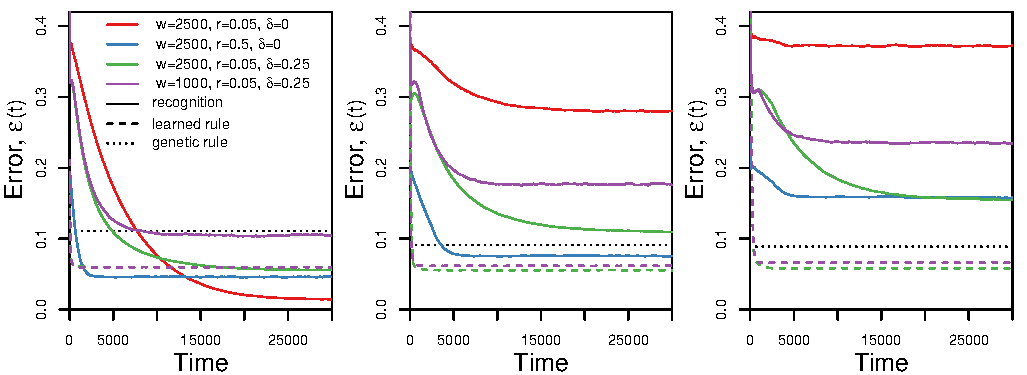
\includegraphics[width=.95\textwidth]{figures/learning_curves.pdf}
\caption{\label{learning_curves} \sffamily\small\textbf{Examples of how average error decreases over time.}
In each panel, we show time in number of interactions on the x-axis and average error, $\bar{\epsilon}$, on the y-axis. The line shows the average error across all animals in all groups and the shaded area shows this average $\pm 0.5$ the standard deviation of error across all animals in all groups. In each panel, blue lines show animals using individual recognition and red lines show animals using the badge system. The solid lines correspond to groups where signal-quality correlation $\rho=0.9$ and the dotted lines correspond to groups where signal-quality correlation $\rho=0.5$. As groups size increases, from A to B, the error of animals using both systems increases, but it affects the error of animals using individual recognition more. As memory window decreases, from B to C, the error of animals using the badge system is not strongly affected, whereas the error of animals using individual recognition becomes higher. Parameters: in all panels $\delta = 0.5$, $\ell_\text{i}=0.2$, $p_\text{o}=0$, $\sigma_\text{b}=0.2$, $\sigma_\text{i}=0.01$, $\sigma_\text{q}=0.5$, $T=10000$; in A $N=20$, $w=2000$; in B $N=50$, $w=2000$; in C $N=50$, $w=500$. }
\end{figure}

\begin{figure}
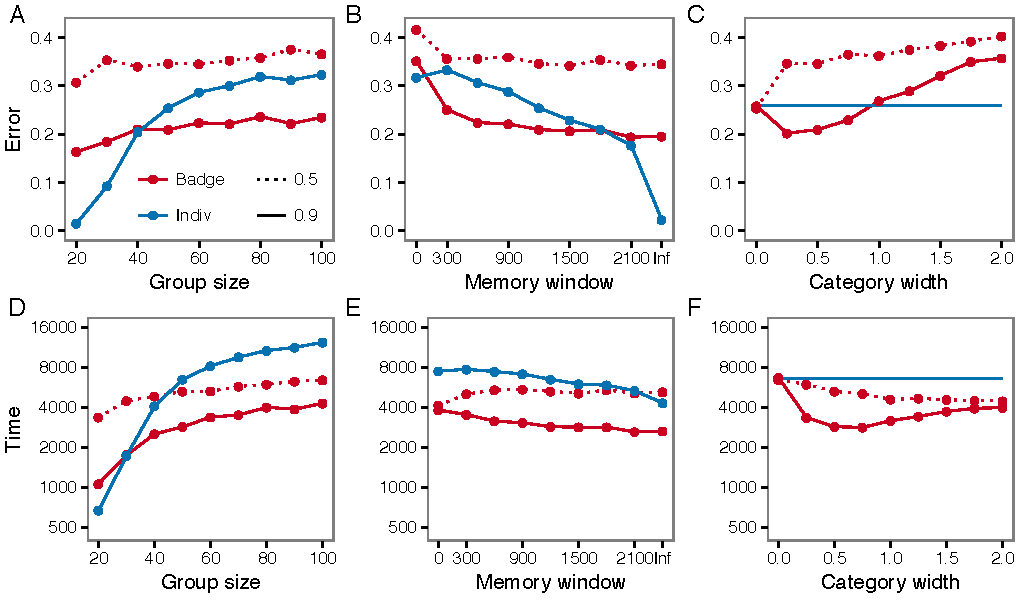
\includegraphics[width=6.85in]{figures/parameters.pdf}
% wait, isn't it decreasing group size and increasing memory that improves memory??
\caption{\sffamily\small\textbf{Increasing[decreasing??] group size and decreasing[increasing??] memory window both improve learning in the absence of observation.} Error and learning time are minimized at an intermediate category width. In the left column, we show average error $\bar{\epsilon}$ as a function of various parameters, and in the right column, we show average learning time $\bar{\tau}$ as a function of various parameters. In each panel, blue lines show animals using individual recognition and red lines show animals using the badge system. The solid red lines correspond to groups in which the signal-quality correlation $\rho=0.9$ and the dotted lines correspond to groups in which the signal-quality correlation $\rho=0.5$. Parameters: unless the parameter is being varied $\delta = 0.5$, $\ell_\text{i}=0.2$, $N=50$, $p_\text{o}=0$, $\sigma_\text{b}=0.2$, $\sigma_\text{i}=0.01$, $\sigma_\text{q}=0.5$, $T=10000$, $w=1100$.}
\label{parameters}
\end{figure}

% Fig 'parameters' description
The effects of group size $N$, memory window $w$, and signal-quality correlation $\rho$ on error and learning time are intuitive and confirm that our model is a reasonable description of a real social system. For animals using both learning systems, smaller groups and longer memory windows make it easier to learn. As group size decreases, both error and learning time decrease (Figure~\ref{learning_curves}A,B; Figure~\ref{parameters}A,B). As memory window increases, error decreases and learning time either slightly decreases or stays constant (Figure~\ref{parameters}B,C). Longer memory windows more effectively reduce error for animals using individual recognition. For animals using the badge system with moderate category widths, they encounter other animals in the same category so often that they rarely forget their opinions before the memory window has elapsed. Only when category width is very small does increasing memory window have a significant effect on error (SI?? Figure~\ref{interactions_badge}). When we compared learning for two badge signals, one with a high badge to quality correlation and one with lower badge to quality correlation, we found that badges with higher correlations with quality always outperformed badges with lower quality correlations (Figure~\ref{parameters}, solid vs dashed red lines). Animals using the badge system learn more accurately and more quickly when the the signal and quality are more strongly correlated.

While changing any of these first three parameters (group size, memory window, and correlation)  either increased or decreased both error and learning time, changing category width led to a tradeoff between error and learning time, increasing one while decreasing the other. Increasing category width results in low learning time and high error (Figure~\ref{parameters}). When a focal animal lumps many of its peers together, it updates its opinion about each of those animals more frequently and by chance may at any given point in time have an accurate opinion about one of the animals in the category, leading to a lower average learning time. On the other hand, by lumping many animals into the same category, it loses its ability to accurately learn about their individual quality values, leading to a higher average error. When the signal-quality correlation is poor, decreasing category width decreases error, by allowing animals to distinguish between their peers more easily. However, when the signal is highly correlated with quality, an intermediate category width minimizes error (Figure~\ref{parameters}). When the signal is a good indicator of quality, it is advantageous to lump animals with similar signals together because it makes sense to transfer information about one of their quality values to other animals in the category. This effect is weakened when the memory window is very long because in that case one can simply learn about all the other animals without a chance of forgetting what has been learned (Figure~\ref{interactions_badge}).
%
\subsection*{The effect of observational learning}
Observational learning helps animals using both systems to learn more accurately and more quickly, but it helps animals using individual recognition much more (Figure \ref{observational}). Observational learning increases the number of animals about which a focal animal can learn at any given time. 
%Since animals using the badge system already learn about multiple animals at once, increasing the probability of observing interactions does not help much. 
In fact, for animals using individual recognition, the same level of error can be achieved by increasing the probability of observing ($p_\text{o}$), by increasing memory window ($w$), or by increasing both to a lesser degree. The same is true of learning time. This can be seen in the strong interaction in how error and learning time change as a function of the probability of observing ($p_\text{o}$) and memory window ($w$) (Figure~\ref{observational}).


\begin{figure}
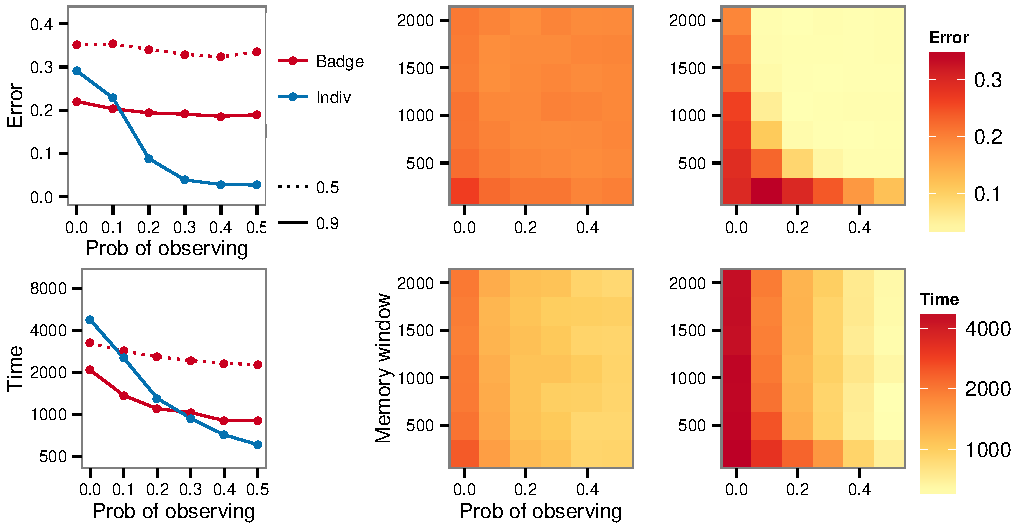
\includegraphics[width=6.85in]{figures/observational_learning.pdf}
\caption{\sffamily\small\textbf{Observational learning improves both error and learning time and does so much more for animals using individual recognition.} For animals using individual recognition, there is a strong interaction between the probability of observing and memory window. In A and D, we show average error $\bar{\epsilon}$ and average learning time $\bar{\tau}$ respectively as a function of the probability of observing, $p_\text{o}$. In each panel, blue lines show animals using individual recognition and red lines show animals using the badge system. The solid red lines correspond to groups in which the signal-quality correlation $\rho=0.9$ and the dotted lines correspond to groups in which the signal-quality correlation $\rho=0.5$. In B and C we show average error $\bar{\epsilon}$ of animals using the badge system and individual recognition respectively as a function of both the probability of observing $p_\text{o}$ on the horizontal axis and memory window $w$ on the vertical axis. In E and F we show average learning time $\bar{\tau}$ of animals using the badge system and individual recognition respectively as a function of both the probability of observing $p_\text{o}$ on the horizontal axis and memory window $w$ on the vertical axis.  Parameters: in all panels $\delta = 0.5$, $\ell_\text{i}=0.2$, $\ell_\text{o}=0.2$, $N=50$, $\sigma_\text{b}=0.2$, $\sigma_\text{i}=0.01$, $\sigma_\text{o}=0.01$, $\sigma_\text{q}=0.5$, $\rho=0.9$, $T=10000$; in A and D $w=1100$, in B and E $\rho=0.9$.}
\label{observational}
\end{figure}

%
\subsection*{Cost of learning}
%I think we should more clearly specify if this is with or without observation
% 
Since increasing group size increases both error and learning time (Figure~\ref{parameters}A,B), it also increases the overall cost of using both learning systems (Figure~\ref{costs}A). The effects of memory window ($w$) and category width ($\delta$) on overall cost depend on the cost function, specifically on the parameter $\alpha$ (Figure \ref{costs}B,C). When $\alpha<1$, the costs of memory window ($c_w$) and category width ($c_\delta$) increase most quickly at low cognitive ability; when $\alpha>1$, the costs of memory window and category width increase most quickly at high cognitive ability (Figure~\ref{cost_fx}). 

When the costs of the memory window increase quickly at low $w$ ($\alpha<1$), the rapid increase in the cost of using a longer memory window is almost exactly offset by the decrease in error and learning time, so the costs of using both systems are almost a constant function of memory window (Figure~\ref{costs}B). However, when the cost of memory window increases quickly at high $w$ ($\alpha>1$), overall costs initially decrease as $w$ increases because of the improvement in error and learning time and only eventually increase because of the cost of using a longer memory window, so an intermediate memory window is the least costly (Figure~\ref{costs}B).

Using a category width $\delta$ equal to $0$ is always costly because it leads to high error and learning time, as we saw above (Figure~\ref{parameters}E,F).  When the costs of category width increase quickly as $\delta$ decreases from $2$ ($\alpha<1$), overall costs tend to increase as $\delta$ decreases, but there is a large range of intermediate $\delta$ at which overall costs are nearly constant: in this range, the increase in cost from decreasing $\delta$ is offset by a decrease in cost from reduced error and learning time. When the costs of category width increase only at low $\delta$ ($\alpha>1$), at first decreasing $\delta$ decreases overall cost by improving error and learning time and only at low $\delta$ does overall cost increase because of the higher cost of this cognitive ability: an intermediate category width is favored (Figure \ref{costs}C).

The overall costs of using the badge system are higher than the costs of using individual recognition when group size is small and memory window is long (Figure~\ref{comparison}A,C). In these cases, animals using individual recognition are capable of learning accurately about their peers and there is no benefit from grouping animals together into categories. When the signal-quality correlation is high, individual recognition is only better for very small groups and very long memory windows (Figure~\ref{comparison}C). 

At an intermediate group size ($N=50$), animals using individual recognition perform similarly to or better than animals using the badge system when category width is small and memory window is long (Figure \ref{comparison}B,D). In these cases, animals using the badge system are paying high costs for their cognitive abilities without receiving much benefit from either improved error or improved learning time. When the signal-quality correlation is high, individual recognition is more costly except when category width is equal to $0$ and the two systems are equivalent (Figure~\ref{comparison}D). 

\begin{figure}
%I think we should more clearly specify if this is with or without observation
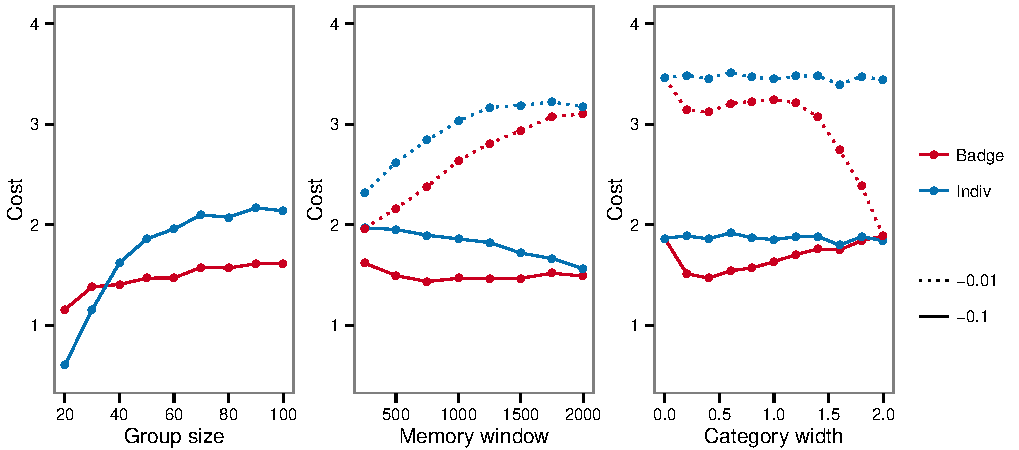
\includegraphics[width=6.85in]{figures/costs.pdf}
\caption{\sffamily\small\textbf{Overall costs are lowest in small groups and with intermediate memory window and category width, when costs increases at high cognitive abilities ($\alpha>1$).} When costs increase at low cognitive abilities ($\alpha<1$), memory window $w$ does not affect overall costs and large category width $\delta$ minimizes overall costs. In A,B, and C, we show overall costs $C$ as a function of group size $N$, memory window $w$, and category width $\delta$ respectively. In each panel, blue lines show animals using individual recognition and red lines show animals using the badge system. The solid lines correspond to $\alpha=5$ and the dotted lines correspond to $\alpha=0.2$.  Parameters: unless the parameter is being varied $\delta = 0.5$, $\ell_\text{i}=0.2$, $N=50$, $p_\text{o}=0$, $\rho=0.9$, $\sigma_\text{b}=0.2$, $\sigma_\text{i}=0.01$, $\sigma_\text{q}=0.5$, $T=10000$, $w=1100$.}
\label{costs}
\end{figure}

\begin{figure}
%I think we should more clearly specify if this is with or without observation
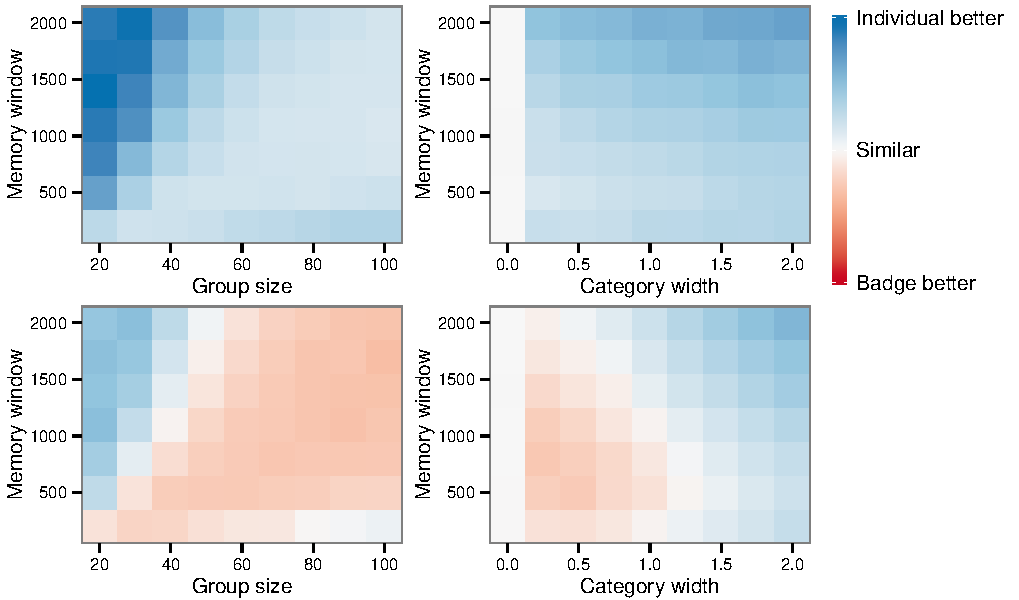
\includegraphics[width=6.85in]{figures/cost_comparisons.pdf}
\caption{\sffamily\small\textbf{The overall costs of using individual recognition are lower than the costs of using the badge system at low group size, high memory window, and low category width.} When the signal-quality correlation $\rho$ increases, animals using the badge system incur lower costs for more combinations or parameters. Here we show the difference in the overall costs ($C$) associated with individual recognition and with the badge system as a function of A,C group size $N$ and memory window $w$ and B,D category width $w$ and memory window $w$. Red indicates the badge system is less costly and blue indicates individual recognition is less costly. Parameters: in A and B $\rho=0.5$, in C and D $\rho=0.9$; unless the parameter is being varied $\delta = 0.5$, $\ell_\text{i}=0.2$, $N=50$, $p_\text{o}=0$, $\sigma_\text{b}=0.2$, $\sigma_\text{i}=0.01$, $\sigma_\text{q}=0.5$, $T=10000$, $w=1100$.}
\label{comparison}
\end{figure}

%%%%%%%%%%%%%%%%%
\section*{Discussion}
%%%%%%%%%%%%%%%%%

% Study question, restated/reframed
Accurate assessment of the quality of conspecifics is important in many contexts, but the conditions under which different assessment systems may be favored is not well understood. Here, we modeled quality assessment in social groups, where agents used either a categorical badge signal (group others into quality categories based on the intensity of badge signals) or an individual recognition system (use individual recognition to remember the outcome of events with particular individuals to estimate quality). Our goal was to better understand the costs and benefits of each system and the conditions under which each system might be favored. 

\subsection*{Summary of results (no costs) and implications} %temporary heading
In the absence of observational learning, our simulations are consistent with general intuition: smaller groups and longer memory duration makes it easier to learn in both learning systems, and agents using the badge system learned more quickly and accurately when there was a strong correlation between the signal and quality. In both systems, we found that increasing the size of the social group and decreasing the duration of each agent's memory window generally caused a nonlinear increase in the extent of assessment errors and the overall time required to learn the quality of others. However, the extent of the impact differed between the two systems. Assessment error and learning time in individual recognition systems were much more affected by increasing group size than the categorical badge system. 

%In the badge system, we also found that changes in the discrimination ability of agents (category width) led to a tradeoff between error and learning time, with increasing category width resulting in lower average learning time but higher error. This is because when a focal animal lumps many of its peers together, it updates its opinion about each of those animals more frequently and by chance may at any given point in time have an accurate opinion about one of the animals in the category, leading to a lower average learning time. On the other hand, by lumping many animals into the same category, it loses its ability to accurately learn about their individual quality values, leading to a higher average error. 

We also found that animals using the badge system could minimize both the error with which they learned and their learning time by having a moderate ability to discriminate between different badges (intermediate category width), as long as the badge was highly correlated with the underlying quality. This is somewhat counterintuitive as one might expect that, if there are no explicit costs to cognition, it should always be advantageous to improve one's cognitive abilities. If that were the case, the explanation of empirical examples of animals with imperfect cognition (e.g. \cite{Kikuchi:2010ys}) would be the costs involved in improving their cognition. However, our results suggest that imperfect cognition itself may be adaptive. Other studies have also found that the most advanced cognitive strategies are not always optimal \cite{Brush:2016kx,Kerr:2003vn,Dunlap:2009vn,Stephens:1991fk}. Our work therefore contributes to our growing understanding of the circumstances that do or do not lead to the evolution of sophisticated cognition.

%also related to a tradeoff between Type I and Type II errors


While a high correlation between quality values and signal values improves the effectiveness of learning via the badge system, our model shows that even with a moderate correlation the badge system is worth using. The correlation values we use are actually a bit higher than those estimated in two of the most frequently cited examples of badge systems, paper wasps and house sparrows\cite{}. Considering the perception of receivers of these quality signals is important, and has a biological basis. For example, in paper wasps, more spots on clypeus means higher dominance \cite{Tibbetts:2004kx} but percentage of black not a significant predictor of dominance \cite{Tibbetts:2004kx}. The critical factor perceived by receivers appears to be the extent to which the black pigment is broken up: more broken means an individual is more dominant. This is somewhat analogous to our more abstract definition of category window size we have used in the current work, where wasps attending to the number of spots could be similar to perceiving a number of categories in signal intensity. 



In the presence of observational learning, agents were able to learn more quickly and accurately in both systems, but the magnitude of this increase differed. Observational learning was more beneficial in improving quality assessments in individual recognition. Observational learning increases the number of animals about which a focal animal can learn at any given time; since animals using the badge system already learn about multiple animals at once, increasing the probability of observing interactions does not have a strong effect on learning rates in badge systems.

\subsection*{Summary of cost results and implications} %temp heading
We found that, depending on how quickly the explicit costs of cognitive traits increase as the traits improve, the costs of using either strategy are minimize by either not investing at all in cognition or investing in a moderate cognitive trait (either memory window or perceptive ability). We found no cases where the benefits of using the most advanced cognitive trait available (either a very long memory window or category width equal to $0$) outweighed the cost of using such a trait. This finding reinforces previous studies XXX that showed how difficult it is for advanced cognition to evolve.



\subsection*{Evolution of assessment systems} %temp heading

Our model results show that the categorical badge system of quality assessment is usually less costly than individual recognition, except when group sizes were small. With a long memory window, systems with a strong correlation between badge and quality showed that individual recognition was beneficial in group sizes less than about 30-40 individuals; with a weaker correlation between badge and quality, individual recognition was beneficial in even larger groups (up to about 50-60 individuals). %interesting that this is about 50, similar to 'Dunbar's number'?
% [this is currently to results-y, and redundant with above, but I think we need some sort of summary here] --- We also found that when we held group size constant at moderately-sized groups (N=50), the discrimination ability of individuals affected which system was most beneficial, but that this differed with the strength of correlation between the badge and quality. With a strong correlation between badge and quality, the categorical system was always less costly than the individual recognition system, except when category width was 0 and the two systems were equivalent. With a weaker badge to quality correlation, individual recognition outperformed categorical badges for long memory windows and small to moderately-sized perception windows.

% under which kinds of natural conditions should we expect to see 1 system vs another?
``[The individual-recognition] hypothesis is especially relevant for species with moderately sized flocks, in which the probability of repeated encounters between the same individuals is great and the value of being recognized is high (Whitfield 1987). These conditions are rare among breeding house sparrows, whose colonies frequently contain several dozen pairs in a small area and many bachelors that arrive throughout the breeding season (pers. obs.) " \cite{Veiga:1993fk}. Also highlights the need to study group dynamics.

% might want to bring in Dunbar + group sizes here? or maybe earlier in intro?





% Learning, recognition, evolution of cognitive complexity / brain size
Our model results identified a sweet spot that results in lower errors....
 Previous modeling of the evolution of cognitive complexity shows that increases can occur on the scale of 10-20 generations (Gavrilets \& Vose 2006 - the dynamics of Machiavellian intelligence) <<ABSTRACT QUOTE:...our results suggest that the mechanisms underlying the ‘‘Machiavellian intelligence’’ hypothesis can indeed result in the evolution of significant cognitive abilities on the time scale of 10 to 20 thousand generations. We show that cerebral capacity evolves faster and to a larger degree than learning ability. Our model suggests that there may be a tendency toward a reduction in cognitive abilities (driven by the costs of having a large brain) as the reproductive advantage of having a large brain decreases and the exposure to memes increases in modern societies.>>
 
\subsection*{Future steps and Conclusion}
By studying a rather simple model, we were able to identify the conditions under which each system is most effective and under which one or the other system should evolve. There are further steps towards improving the realism of the model that will also improve our predictions about the evolution of the two learning strategies. XXX

Our study shows that is not enough to study the conditions that could allow for the evolution of a particular type of learning. By considering and comparing two solutions to the same biological problem we find that different conditions favor different solutions. %%Eleanor just wrote this and knows it needs work! 
 
 
%%%%%%%%%%%%%%%%%%%%% previous notes %%%%%%%%%%%%%%%%%
% Result 3: number of categories in badge systems
While a high correlation between quality values and signal values improve the effectiveness of learning via the badge system, our model shows that even with a moderate correlation the badge system is worth using. The correlation values we use are actually a bit higher than those estimated in two of the most frequently cited examples of badge systems, paper wasps and house sparrows.

paper wasps: more spots on clypeus means higher dominance \cite{Tibbetts:2004kx} but percentage of black not a significant predictor of dominance \cite{Tibbetts:2004kx}. what really matters is ``brokenness" of black pigment: more broken means more dominance. But could we say that paying attention to number of spots is like a rough number of categories? 





examples of cases where maximal cognitive abilities are not optimal
\cite{Kerr:2003vn,Stephens:1991fk,Brush:2016kx,Dunlap:2009vn} 

real observation of imperfect cognition in predators of coral snakes \cite{Kikuchi:2010ys}

empirical examples of badges: black on face of paper wasps \cite{Tibbetts:2004kx}, house sparrows \cite{Veiga:1993fk}, black crowns on swamp sparrows \cite{Olsen:2010uq}

 swamp sparrows: black crown --> aggression, less black crown --> parental care 
 
 S Rohwer. Social significance of avian winter plumage variability for black-aggression correlation. Evolution. 1975.
 
 Siefferman L and Hill GE. Structural and melanin coloration indicate parental effort and reproductive success in male eastern bluebirds. Behavioral Ecology. 2003. for coloration-parental care correlation
 
 Bokony V and Liker A. Melanin-based black plumage coloration is related to reproductive investment in cardueline finches. Condor. 2005. for coloration-parental care correlation
 
paper wasps: more spots on clypeus means higher dominance \cite{Tibbetts:2004kx} but percentage of black not a significant predictor of dominance \cite{Tibbetts:2004kx}. what really matters is ``brokenness" of black pigment: more broken means more dominance. But could we say that paying attention to number of spots is like a rough number of categories? 

While a high correlation between quality values and signal values improve the effectiveness of learning via the badge system, our model shows that even with a moderate correlation the badge system is worth using. The correlation values we use are actually a bit higher than those estimated in two of the most frequently cited examples of badge systems, paper wasps and house sparrows.

paper wasps: head width-percentage black $r^2=0.36$ for wasps with at least 2 spots, ``badge brokenness was the only significant predictor of dominance when included with spot number and percentage of clypeus black in a multiple logistic regression (whole model, $r^2=0.105$)  \cite{Tibbetts:2004kx} 

house sparrows: badge size is correlated with physical condition $r=0.379$ \cite{Veiga:1993fk}

swamp sparrow: rusty cap is correlated with parental investment ($r^2=0.33$) and black forehead is correlated with aggression (negative correlation with distance to intruder $r^2=0.41$) \cite{Olsen:2010uq}

``[The individual-recognition] hypothesis is especially relevant for species with moderately sized flocks, in which the probability of repeated encounters between the same individuals is great and the value of being recognized is high (Whitfield 1987). These conditions are rare among breeding house sparrows, whose colonies frequently contain several dozen pairs in a small area and many bachelors that arrive throughout the breeding season (pers. obs.) " \cite{Veiga:1993fk}. Also highlights the need to study group dynamics.

Whitfield, D. P. 1986. Plumage variability and territoriality in breeding turnstone: status signalling or individual recognition? Animal Behaviour.

Whitfield, D. P. 1987. Plumage variability, status signalling, and individual recognition in avian flocks. Trends in Ecology and Evolution.




\newpage
\bibliography{BIB_badgeVSrecog,TODO_newrefs, Mendeley_Badge_vs_Recognition.bib}
\bibliographystyle{apa}

\section{Supplemental Information } 
\begin{figure}[h]
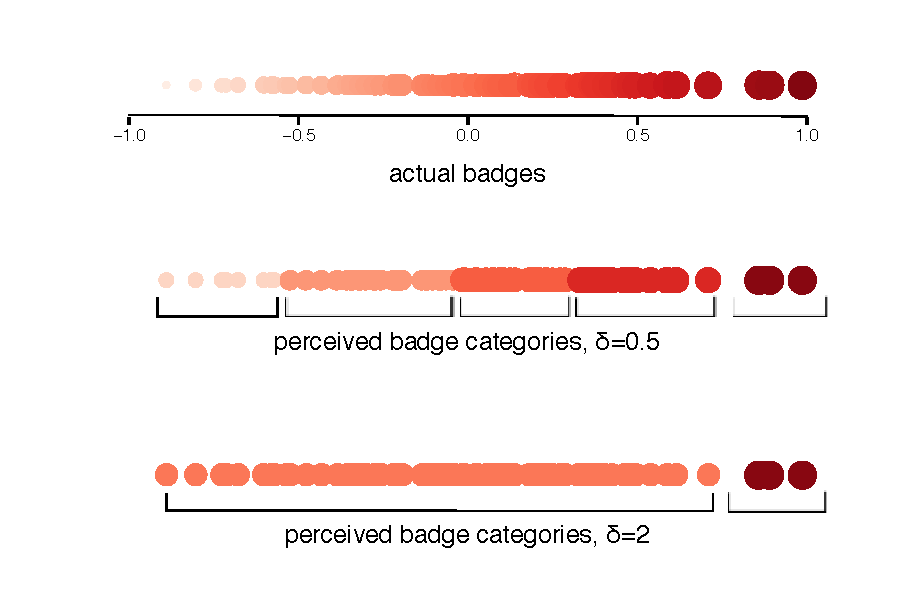
\includegraphics[width=.8\textwidth]{figures/categories.pdf}
\caption{\sffamily\small\textbf{Example of how categories are defined.}
Here we show how a group of size $N=40$ might be divided into categories with maximum width $0.5$. Each point corresponds to an animal in the group. We show the signal of each animal on the y-axis and the order of the animals from lowest to highest signal on the x-axis. The color of the point indicates the category to which it belongs and the horizontal lines show the median signal value for each category. Categories were formed by choosing an animal $i$ at random, putting all other animals whose signals were within $\delta/2$ of $i$'s signal $s_i$ into the same category, then choosing another uncategorized animal at random, and continuing until all animals were categorized.}
 \label{cats_ex}
\end{figure}

\begin{figure}[h]
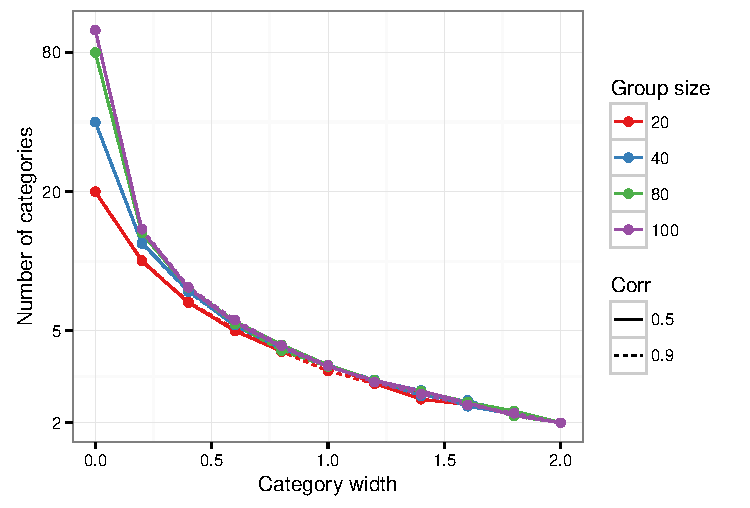
\includegraphics[width=.8\textwidth]{figures/number_of_categories.pdf}
\caption{\sffamily\small\textbf{As category width $\delta$ decreases the number of categories into which the group is divided increases.}
For a given group size $N$ and category width $\delta$ we generated a group with $N$ signal values $\{s_i\}$ and categorized the group according to the procedure in the text and Figure \ref{cats_ex} $100$ times and took the average number of categories across these $100$ groups. Here we show how the average number of categories into which a group is divided depends on group size $N$ and category width $\delta$.  Each colored line corresponds to a group size. There are overlapping solid and dotted lines in each color since the signal-quality correlation $\rho$ does not affect the number of categories formed. When $\delta=0$ there are as many categories as there are animals in the group. When $\delta=2$ there are on average $2$ categories, although it can happen that all animals are put into the same category. }
\label{num_cat}
\end{figure}

\begin{figure}[h]
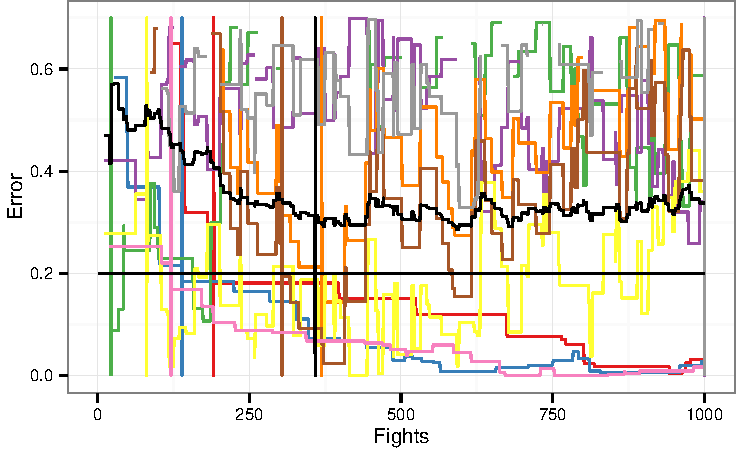
\includegraphics[width=.8\textwidth]{figures/learning_time_example.pdf}
\caption{\label{learnT.ex} \sffamily\small\textbf{Example of how to calculate learning time.} Learning time $\tau_i$ can be less than $T$, even if average error at time $T$ is above the threshold $0.2$. Each colored line shows how one the error in one animal's opinion of its five group mates changes over time. The black line is its average error about the other animals, $\epsilon_i(t)$. The horizontal black line is the error threshold, $0.2$. Each vertical colored line is the first time when corresponding line drops below the threshold. The vertical black line is the average of these learning times, $\tau_i$.}
\end{figure}

\begin{figure}[h]
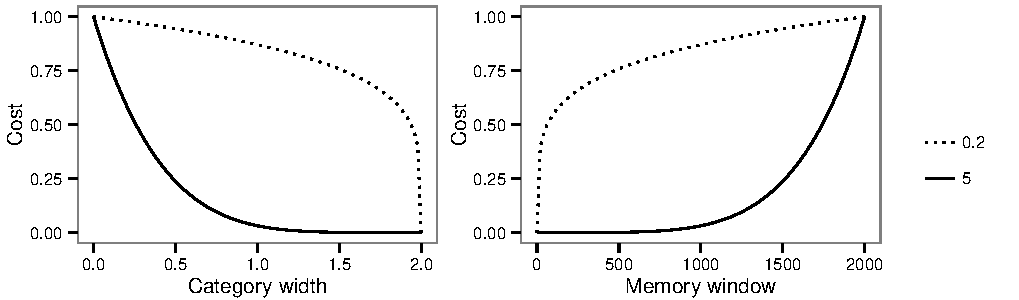
\includegraphics[width=.8\textwidth]{figures/cost_functions.pdf}
\caption{\sffamily\small\textbf{Cost functions.} Here we show how the cost functions for the cognitive parameters category width and memory window. In each panel, the solid line corresponds to $\alpha=5$ and the dotted line corresponds to $\alpha=0.2$. }
\label{cost_fx}
\end{figure}

\begin{figure}[h]
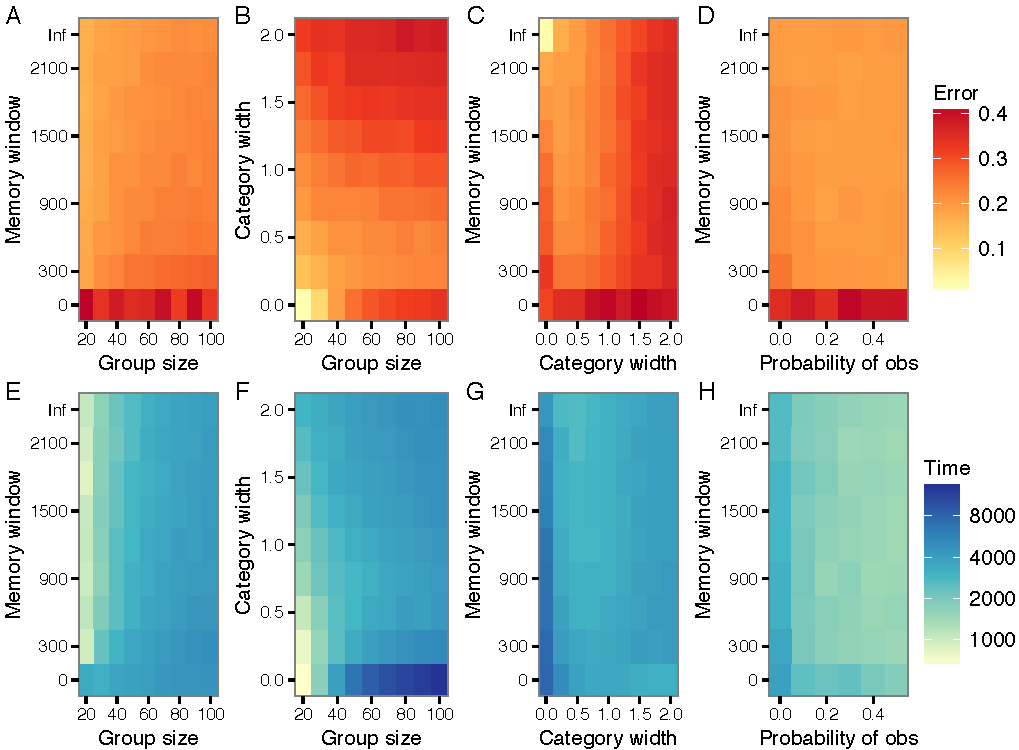
\includegraphics[width=.8\textwidth]{figures/parameter_interactions_badge.pdf}
\caption{\sffamily\small\textbf{Parameter interactions for animals using the badge system.}
In A, B, and C we show average error $\bar{\epsilon}$ for animals using the badge system as a function of two parameters. In D, E, and F we show average learning time $\bar{\tau}$ as a function of two parameters. Parameters: unless the parameter is being varied $\delta = 0.5$, $\ell_\text{i}=0.2$, $N=50$, $p_\text{o}=0$, $\rho=0.9$, $\sigma_\text{b}=0.2$, $\sigma_\text{i}=0.01$, $\sigma_\text{q}=0.5$, $T=10000$, $w=1100$.}
\label{interactions_badge}
\end{figure}

\begin{figure}[h]
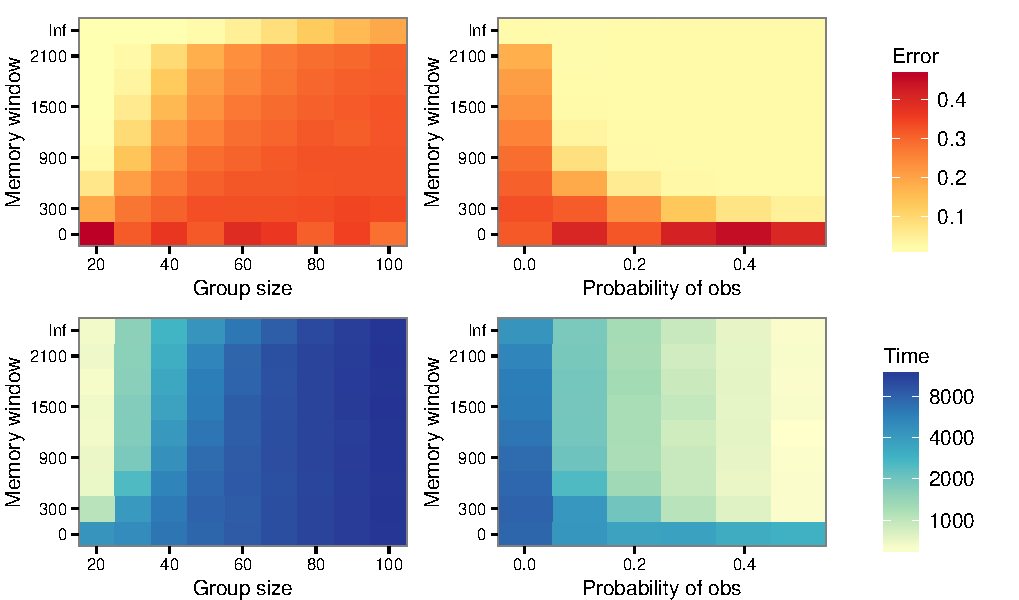
\includegraphics[width=.8\textwidth]{figures/parameter_interactions_indiv.pdf}
\caption{\sffamily\small\textbf{Parameter interactions for animals using individual recognition.}
In A, B, and C we show average error $\bar{\epsilon}$ for animals using individual recognition as a function of two parameters. In D, E, and F we show average learning time $\bar{\tau}$ as a function of two parameters. Parameters: unless the parameter is being varied $\delta = 0.5$, $\ell_\text{i}=0.2$, $N=50$, $p_\text{o}=0$, $\rho=0.9$, $\sigma_\text{b}=0.2$, $\sigma_\text{i}=0.01$, $\sigma_\text{q}=0.5$, $T=10000$, $w=1100$.}
\label{interactions_indiv}
\end{figure}
\end{document}

% CUT TEXT

% summary data quantified
We then use the simulated interaction datasets to quantify: 
\begin{enumerate}
  \item Learning curves: each individual's opinion error across the series of fights 
  \item Learning accuracy: amount of error in final opinions about quality (summarize histograms of learning error)
  \item Learning time: amount of fights (time) for opinion to achieve maximum potential accuracy (opinion at end of all fights)  
\end{enumerate}